%近畿大学理工学部情報学科卒業論文雛形兼論文作成の手引き
% ver 0.1 2005/11/28 by Toru Kato
% ver 0.2 2006/11/28 by Takashi Ishimizu
% ver 0.3 2007/11/26 by Toru Kato
% ver 0.4 2008/12/14 by Shoji Mizobuchi
% ver 0.5 2011/12/1 by Sen Moriya

\documentclass{jsarticle}
\usepackage[dvipdfmx]{graphicx}
\usepackage{url}

\begin{document}
\pagestyle{empty}

\begin{center}
\vspace*{1cm}
\large
{\LARGE 卒業研究報告書}\\
\vspace*{0.8cm}
題目\\
\vspace*{1cm}
{\Huge \underline{研究題名をここに書く}}\\
\vspace{3mm}
{\LARGE \underline{副題があればここに書く}}\\

\vspace*{3cm}
指導教員\\
\vspace*{0.3cm}
\underline{\LARGE 卒山 研 講師}\\
%\vspace*{-0.3cm}
%\underline{\hspace*{5cm}}\\
\vspace*{3cm}
報告者\\
\vspace*{0.3cm}

{XX--1--037--0999}\\
\vspace*{0.3cm}
\underline{\Huge 近大 情治}\\
% \vspace*{-0.3cm}
% \underline{\hspace*{5cm}}\\
\vspace*{0.5cm}
近畿大学理工学部情報学科\\
\vspace*{2cm}
令和XX年Y月Z日提出\\
\end{center}

\newpage
\normalsize


%\tableofcontents
\clearpage
\begin{center}
{\bf \Large 概要}
\end{center} 

本研究の目的,内容の要点を,半ページ~1ページを目安に記述する.
□□□□□□□□□□□□□□□□□□□□□□□□□□□□□□
□□□□□□□□□□□□□□□□□□□□□□□□□□□□□□
□□□□□□□□□□□□□□□□□□□□□□□□□□□□□□
□□□□□□□□□□□□□□□□□□□□□□□□□□□□□□
□□□□□□□□□□□□□□□□□□□□□□□□□□□□□□
□□□□□□□□□□□□□□□□□□□□□□□□□□□□□□
□□□□□□□□□□□□□□□□□□□□□□□□□□□□□□
□□□□□□□□□□□□□□□□□□□□□□□□□□□□□□
□□□□□□□□□□□□□□□□□□□□□□□□□□□□□□
□□□□□□□□□□□□□□□□□□□□□□□□□□□□□□
□□□□□□□□□□□□□□□□□□□□□□□□□□□□□□
□□□□□□□□□□□□□□□□□□□□□□□□□□□□□□
□□□□□□□□□□□□□□□□□□□□□□□□□□□□□□
□□□□□□□□□□□□□□□□□□□□□□□□□□□□□□
□□□□□□□□□□□□□□□□□□□□□□□□□□□□□□
□□□□□□□□□□□□□□□□□□□□□□□□□□□□□□
□□□□□□□□□□□□□□□□□□□□□□□□□□□□□□
□□□□□□□□□□□□□□□□□□□□□□□□□□□□□□
□□□□□□□□□□□□□□□□□□□□□□□□□□□□□□
□□□□□□□□□□□□□□□□□□□□□□□□□□□□□□
□□□□□□□□□□□□□□□□□□□□□□□□□□□□□□
□□□□□□□□□□□□□□□□□□□□□□□□□□□□□□
□□□□□□□□□□□□□□□□□□□□□□□□□□□□□□
□□□□□□□□□□□□□□□□□□□□□□□□□□□□□□
□□□□□□□□□□□□□□□□□□□□□□□□□□□□□□
□□□□□□□□□□□□□□□□□□□□□□□□□□□□□□
□□□□□□□□□□□□□□□□□□□□□□□□□□□□□□
□□□□□□□□□□□□□□□□□□□□□□□□□□□□□□
□□□□□□□□□

\newpage

\tableofcontents
\newpage
\setcounter{page}{1}
\pagestyle{plain}

\section{序論}\label{sec1}
\subsection{本研究の背景}
関連分野の動向等,本研究を始めるにあたって調査した内容をまとめる.

\subsection{本研究の目的}
本研究では何を目的とし,どのような事柄を明らかにするのか,あるいは
どのような問題を解決するのかをまとめる.

\subsection{本報告書の構成}
2節以降の各節の内容を簡潔に記述する.

\section{研究内容}\label{sec2}
研究についての具体的な内容を2節以降で記述する.
各節のタイトルは任意.ただし結論,今後の課題,謝辞,参考文献など,論文
としての常識的な項目は必ず入れなければならない.詳しくは卒業研究
担当教員の指導に従うこと.


\subsection{図,表のキャプションと参照}

図や表には必ず題名と参照番号を記述すること.参照番号はlabel を使って自
動的に作成するようにし,ref を使って本文中で参照できるようにしておく.

\begin{figure}[htbp]
  \begin{center}
     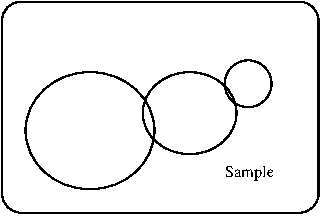
\includegraphics[width=13cm,height=12cm,keepaspectratio]{figure.pdf}\\
     %includegraphicsの詳しい使い方ははLaTeXの参考書を参照.
  \end{center}
  \caption{図の例}%
\label{fig1}
\end{figure}

図や表を入れた場合,必ず図の参照番号を使った文章が本文中にあるはずである.例えば
次のようにすればよい.図\ref{fig1} は図のサンプルである.\TeX のソース
を見ると図の入れ方がわかる.

図が単独で現れ,本文中に何の説明もなければ,ただのページ稼ぎと見なされ
る.

\subsection{参考文献の引用}
参考文献は,本研究が十分な調査活動を基礎として成り立っていることを
明示する,大変重要な項目である.
研究で参考とした文献のリストを論文の終わりに入れ,
それらの文献に関係のある記述部分や,文献に書いてある文章の引用を本文内で行なって
ある箇所には必ず参考文献の番号を入れなければならない.例えば次のよう
にすれば良い.本手引きや予稿の手引きを作成する際,文献
\cite{kinosita}を参考にした.また\LaTeX の各種コマンドに関する説
明は文献\cite{okumura}を参考にした.\TeX \cite{knuth} とは,Knuth によっ
て作られた組版用のソフトウェアのことである.文献\cite{labelName}は,論
文を参照する場合のサンプルである.



本手引き書ではbibitem を用いて直接参考文献リストを本文末尾に記入してい
るが,出来れば文献データベースから参考文献リストを自動的に作成する
\BibTeX 等を使用した方が良い.本手引書の\LaTeX ソースと共に,\BibTeX の
データベースファイルも配布する.\BibTeX の詳しい使用方法については,
文献\cite{okumura}等\LaTeX の参考書を参照のこと.

\subsection{各節の引用}
各節にも label をつけておいて,後の節で節番号を使って自動的に引用番号
を記述できるようにしておくと良いだろう.例えば次のようにすれば良い.
\ref{sec1}節で述べた目的を達成するため,本節では次のような方法を用いた
場合につい述べる.$\cdots$

label とref を用いた参照は 図のキャプションや section, subsection だけ
でなく,数式等にも使えるので,番号を手でつけることは出来るだけ控え,
自動的な番号づけと参照を行ない間違いのない文章になるようにしよう.



\section{結論・今後の課題}
本報告書の結論や,研究の過程で明らかになった今後の課題等を記述する.

\newpage
\section*{謝辞}
\addcontentsline{toc}{section}{謝辞}% 追加
指導を受けた教員や,本研究を完成するにあたって支援を受けた研究室の諸氏
に対しお礼の言葉を,独立したページに記述する.詳しくは卒業研究
担当教員の指導に従うこと.


\newpage

%jbibtexを使う場合は,以下の「%ここから」「%ここまで」をコメントアウトし,

%%ここから
\begin{thebibliography}{1}
\addcontentsline{toc}{section}{\refname}% 追加
\bibitem{knuth}
Donald E Knuth. The \TeX book. Addison--Wesley, 1986.

\bibitem{kinosita}
木下是雄. 理科系の作文技術. 中公新書 624, 1981.


\bibitem{okumura}
奥村晴彦. [改訂第4版] \LaTeXe 美文書作成入門. 技術評論社, 2007.

\bibitem{labelName}
第1著者, 第2著者.
\newblock 論文名(論文の場合のかき方).
\newblock 論文誌名, 巻番号, 号番号, pp. 31--38, 2018.


\end{thebibliography}
%%ここまで

%そして以下の2行: \bibliography{reference} と
%\addcontentsline{toc}{section}{\bibname}のコメントアウトを解除する.

%\addcontentsline{toc}{section}{\bibname}
%\bibliography{reference}

\bibliographystyle{jplain}

\newpage
\appendix
\section{付録について}
本研究で作成したプログラムのソースファイルなどを卒業研究報告書に含めた
い場合は,付録として巻末にまとめておく.

\end{document}
 

%%% Local Variables: 
%%% mode: latex
%%% TeX-master: t
%%% End: 
